%  !TeX  root  =  user_guide.tex
% % \section{Working with Raster Data}\label{label_raster}
\chapter{Les données raster}\label{label_raster}
\index{couches raster|(}

% when the revision of a section has been finalized, 
% comment out the following line:
%\updatedisclaimer

% This Section describes how to visualize and set raster layer properties.
% \qg supports a number of different raster formats. Currently tested formats
% include:\index{raster layers!data formats}

Cette section explique comment visualiser et définir les propriétés d'une couche raster.
\qg utilise la bibliothèque GDAL pour lire et écrire des données en format raster
\footnote{La gestion des rasters de GRASS est réalisée par une extension de source de données native.}, contenant Arc/Info Binary Grid\index{Arc/Info Binary Grid}, 
Arc/Info ASCII Grid\index{Arc/Info ASCII Grid},GeoTIFF\index{GeoTIFF},
Erdas Imagine\index{Erdas Img.} et beaucoup plus.

A ce jour plus de 100 formats raster sont supportés par la bibliothèque GDAL \cite{GDALweb}.
Une liste complète est disponible sous \url{http://www.gdal.org/formats_list.html}.

\textbf{Note}: Pas tous les formats listés ne fonctionnent avec QGIS pour différentes raisons.
Par exemple, certains nécessitent des bibliothèques commerciales externes ou l'installation GDAL de votre OS n'a pas été conçue pour supporter le format que vous souhaitez utiliser.
Seuls les formats qui ont été testés apparaissent dans la liste des types de fichier au moment
du chargement des données raster dans QGIS. D'autres formats non testés  peuvent être chargés
en sélectionnant *.*.

Le traitement des données raster avec GRASS est décrit dans la section \ref{sec:grass}.

% \section{What is raster data?}\label{label_whatsraster}
\section{Que sont les données raster ?}\label{label_whatsraster}
\index{couches raster !définition}

% Raster data in GIS are matrices of discrete cells that represent features on,
% above or below the earth's surface. Each cell in the raster grid is the same
% size, and cells are usually rectangular (in \qg they will always be
% rectangular). Typical raster datasets include remote sensing data such as
% aerial photography or satellite imagery and modelled data such as an elevation
% matrix.
Les données rasters dans les SIG sont des matrices de cellules discrètes qui
représentent des objets, au-dessus ou en dessous de la surface de la Terre.
Chaque cellule dans la grille raster est de la même taille et les cellules sont
généralement rectangulaires (dans \qg elles seront toujours rectangulaires).
Un jeu de données raster typique inclut les données des capteurs distants
telles que les photographies aériennes ou les images de satellites et les
données modélisées telles que les matrices d'élévation.

% Unlike vector data, raster data typically do not have an associated database
% record for each cell. They are geocoded by its pixel resolution and the x/y 
% coordinate of a corner pixel of the raster layer. This allows \qg to
% position the cata correctly in the map canvas.
Contrairement aux données vectorielles, les données rasters n'ont typiquement pas de
base de données d'enregistrement associée. Elles sont géocodées par leur
résolution de pixel et leurs coordonnées x/y du coin du pixel de la couche
raster. Cela permet à \qg de positionner les données correctement dans la zone
de la carte.

% \qg makes use of georeference information inside the raster layer (e.g.
% GeoTiff) or in an appropriate world file to properly display the
% data.\index{raster layers!georeferenced}
\qg utilise les informations de géoréférencement dans les couches rasters (par
exemple GeoTiff) ou dans un fichier world approprié pour afficher correctement
les données.\index{couches raster!géoréférencer}

% \section{Loading raster data in \qg}\label{label_loadraster}
\section{Charger des données rasters dans \qg}\label{label_loadraster}

% Raster layers are loaded either by clicking on the 
% \toolbtntwo{mActionAddRasterLayer}{Load Raster} icon or by selecting the 
% \mainmenuopt{View}>\dropmenuopttwo{mActionAddRasterLayer}{Add Raster Layer} 
% menu option. More than one layer can be loaded at the same time by holding
% down the \keystroke{Control} or \keystroke{Shift} key and clicking on multiple
% items in the dialog \dialog{Open a GDAL Supported Raster Data
% Source}.\index{raster layers!loading}
Les couches rasters sont chargées soit en cliquant sur l'icône
\toolbtntwo{mActionAddRasterLayer}{Charger une couche raster} soit en
sélectionnant l'option du menu
\mainmenuopt{Couches}>\dropmenuopttwo{mActionAddRasterLayer}{Ajouter une
couche raster}. Plus d'une couche peut être chargée en même temps en appuyant
sur la touche \keystroke{Control} ou \keystroke{Shift} et en cliquant sur de
plusieurs couches dans la boîte de dialogue\\ \dialog{Ouvrez des sources de
données rasters gérées par GDAL}.\index{couches raster!charger}

% Once a raster layer is loaded in the map legend you can click on the layer
% name with the right mouse button to select and activate layer specific
% features or to open a dialog to set raster properties for the layer.
Une fois la couche raster chargée dans la légende de la carte vous pouvez
cliquer sur le nom de la couche avec le bouton droit de la souris pour
sélectionner et activer des paramètres spécifiques à la couche ou pour ouvrir
une boîte de dialogue pour définir des propriétés du raster pour la couche.

% \minisec{Right mouse button menu for raster layers}
\minisec{Menu du bouton droit de la souris pour les couches raster}

\begin{itemize}[label=--]
% \item \dropmenuopt{Zoom to layer extent}
% \item \dropmenuopt{Zoom to best scale (100\%)}
% \item \dropmenuopt{Show in overview}
% \item \dropmenuopt{Remove}
% \item \dropmenuopt{Properties}
% \item \dropmenuopt{Rename}
% \item \dropmenuopt{Add Group}
% \item \dropmenuopt{Expand all}
% \item \dropmenuopt{Collapse all}
% \item \dropmenuopt{Show file groups}
\item \dropmenuopt{Zoom sur l'étendue de la couche}
\item \dropmenuopt{Zoom à la meilleur échelle (100\%)}
\item \dropmenuopt{L'affiche dans l'aperçu}
\item \dropmenuopt{Supprimer}
\item \dropmenuopt{Définir le SCR d'une couche}
\item \dropmenuopt{Définir le SCR du projet depuis cette couche}
\item \dropmenuopt{Propriétés}
\item \dropmenuopt{Renommer}
\item \dropmenuopt{Ajouter un groupe}
\item \dropmenuopt{Tout éténdre }
\item \dropmenuopt{Tout diminuer}
\item \dropmenuopt{Afficher les groupes du fichier}
\end{itemize}

% \section{Raster Properties Dialog}\label{label_rasterprop}
\section{Boîte de dialogue de propriétés des Rasters}\label{label_rasterprop}

% To view and set the properties for a raster layer, double click 
% on the layer name in the map legend or right click on the layer name and
% choose \dropmenuopt{Properties} from the context menu:\index{raster
% layers!context menu} Figure \ref{fig:raster_properties} shows the
% \dialog{Raster Layer Properties} dialog. There are several tabs on the
% dialog: 
Pour voir et définir les propriétés d'une couche raster, double-cliquez sur le nom de la couche dans la légende de la carte ou cliquez droit sur le nom de la couche et choisissez\\ \dropmenuopt{Propriétés} du menu
contextuel:\index{couche raster!menu contextuel}  Figure
\ref{fig:raster_properties} montre la boîte de dialogue\\ \dialog{Propriétés
de la couche raster}. Il y a plusieurs onglets dans cette fenêtre :

\begin{itemize}[label=--]
%  \item \tab{Symbology}
%  \item \tab{Transparency}
%  \item \tab{Colormap}
%  \item \tab{General}
%  \item \tab{Metadata}
%  \item \tab{Pyramids}
%  \item \tab{Histogram}
 \item \tab{Style}
 \item \tab{Transparence}
 \item \tab{Palette de couleur}
 \item \tab{Général}
 \item \tab{Méta-données}
 \item \tab{Pyramides}
 \item \tab{Histograme}
\end{itemize}

\begin{figure}[htb]
  \begin{center}
%    \caption{Raster Layers Properties Dialog
% \nixcaption}\label{fig:raster_properties}\smallskip
   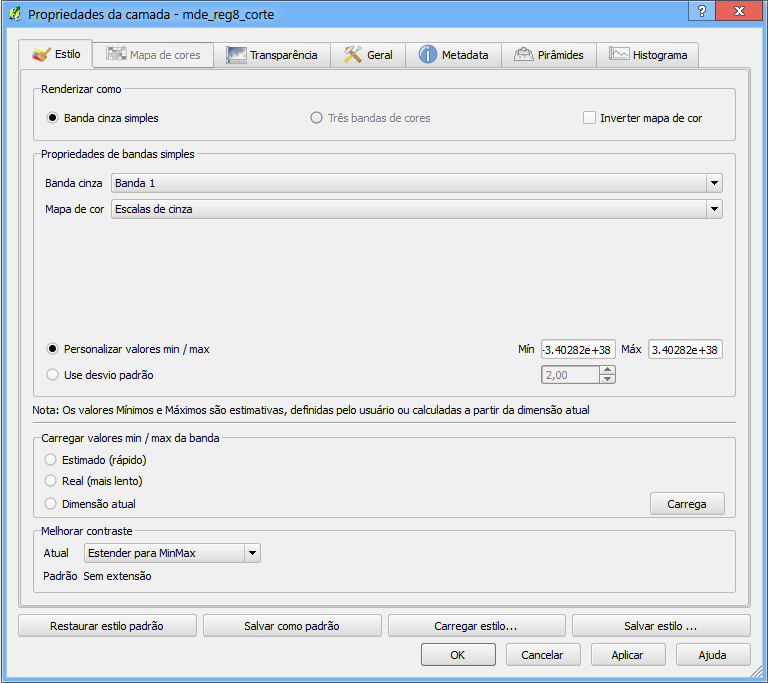
\includegraphics[clip=true, width=10cm]{rasterPropertiesDialog}
   \caption{Boîte de dialogue des propriétés des couches raster
\nixcaption}\label{fig:raster_properties}
\end{center}
\end{figure}

\subsection{Onglet Style}\label{label_sombology}

% \qg can render raster layers in two different ways :\index{raster
% layers!supported channels}
\qg peut afficher des couches rasters de deux manières différentes
:\index{couches layers!canaux gérés}

\begin{description}
% \item Single band - one band of the image will be rendered as gray or in 
% pseudocolors.
\item[Bande unique :] une bande de l'image sera affichée en nuance de gris, en pseudocouleurs ou 
couleurs farfelues.
% \item Three band color - three bands from the image will be rendered, each 
% band representing the red, green or blue component that will be used to
% create a color image.
\item[Trois bandes de couleurs :] trois bandes de l'image seront affichées,
chaque bande représentant le composant rouge, vert ou bleu qui sera utilisé pour créer une image de couleur.
\end{description}

% Within both rendertypes you can invert the color output using the 
% \checkbox{Invert color map} checkbox.
Pour les deux types de rendu, vous pouvez inverser la sortie couleur en
utilisant la case à cocher \checkbox{Inverser la carte de couleur}.

% \minisec{Single Band Rendering}
\minisec{Rendu des bandes simples}

% This selection offers you two possibilites to choose. At first you can
% select which band you like to use for rendering (if the dataset has more than 
% one band).
Ce choix vous permet deux possibilités : vous pouvez d'abord sélectionner
quelle bande vous voulez utiliser pour le rendu (si le jeu de données a plus
d'une bande).

% The second option offers a selection of available colortables for rendering.
La seconde option vous offre une sélection des tables de couleurs disponibles
pour le rendu.

% The following settings are available through the dropdownbox
% \selectstring{color map}{Grayscale}, where grayscale is the default setting.
Les paramètres suivants sont disponibles à travers la liste déroulante\\
\selectstring{carte de couleur}{Niveau de gris}, où niveau de gris est le 
paramètre par défaut.

% Also available are
Sont aussi disponible :
\begin{itemize}[label=--]
% \item Pseudocolor
\item Pseudo-couleur
% \item Freak Out
\item Pseudo-couleur psychédélique
% \item Colormap
\item Palette de couleurs
\end{itemize}

% When selecting the entry \selectstring{color map}{Colormap}, the tab
% \tab{Colormap} becomes available. See more on that at chapter
% \ref{label_colormaptab}.
Quand vous sélectionnez \selectstring{couleurs indexées}{Palette de couleurs}, l'onglet
\tab{Couleurs indexées} est disponible. Plus d'informations dans le chapitre
\ref{label_colormaptab}.

% \qg can restrict the data displayed to only show cells whose values are
% within a given number of standard deviations of the mean for the
% layer.\index{raster layers!standard deviation} This is useful when you have
% one or two cells with abnormally high values in a raster grid that are having
% a negative impact on the rendering of the raster. This option is only
% available for pseudocolor images.
\qg peut restreindre les données affichées pour afficher seulement les
cellules dont la valeur sont dans un nombre donné de déviations standards de la moyenne pour la couche.\index{couches raster!déviation standard} Cela est utile quand vous avez une ou deux cellules avec des valeurs anormalement hautes dans une grille raster qui ont un impact négatif sur le rendu du raster. Cette option est seulement disponible pour les images en pseudocouleur.

% \minisec{Three band color}
\minisec{Couleur à trois bandes}

% This selection offers you a wide range of options to modify the appereance
% of your rasterlayer. For example you could switch color-bands from the
% standard RGB-order to something else.
Cette sélection vous offre un large choix d'options pour modifier l'apparence de votre couche raster. Par exemple, vous pouvez passer les bandes de couleurs d'un ordre standard RVB à un autre.

% Also scaling of colors are available.
L'échantillonnage des couleurs est également disponible.

% \begin{Tip}\caption{\textsc{Viewing a Single Band of a Multiband Raster}}
\begin{Tip}\caption{\textsc{Visualiser une seule bande d'un raster multibande}}
% \qgistip{If you want to view a single band (for example Red) of a multiband
% image, you might think you would set the Green and Blue bands to ``Not
% Set''. But this is not the correct way. To display the Red band, 
% set the image type to grayscale, then select Red as the band to use for Gray.
Si vous désirez visualiser une seule bande (par exemple la bande rouge)
d'une image multibande, vous pouvez penser que vous pourriez définir les bandes Vertes et Bleue à Non définie. Mais ce n'est pas la manière correcte. Pour afficher la bande Rouge définissez le type d'image à nuance de gris, puis sélectionnez Rouge comme bande à utiliser pour le Gris.
\end{Tip} 

% \subsection{Transparency Tab} \label{rastertab:transparency}
\subsection{Onglet transparence} \label{rastertab:transparency}

% \qg has the ability to display each raster layer at varying transparency
% levels.\index{raster layers!transparency} Use the transparency slider to
% indicate to what extent the underlying layers (if any) should be visible
% though the current raster layer. This is very useful, if you like to overlay
% more than one rasterlayer, e.g. a shaded relief-map overlayed by a classified
% rastermap. This will make the look of the map more three dimensional.
\qg a la possibilité d'afficher chaque raster à des niveaux de transparence
différents.\index{couches raster!transparence} Utiliser la barre coulissante de transparence pour indiquer à quel niveau de transparence les couches sous-jacentes (s'il y en a) pourront être visible à travers cette couche raster. Cela est très utile, si vous désirez superposer plus d'une couche raster, par exemple une carte des reliefs ombrés superposée par une carte raster classifiée. Cela rendra la carte encore plus proche de la troisième dimension.

% Additionally you can enter a rastervalue, which should be treated as
% {\em NODATA}. This can be done manually or with the 
% \toolbtntwo{mActionContextHelp}{Add values from display} icon.
De plus, vous pouvez entrer une valeur raster qui pourra être traitée comme {\em NODATA}. Cela peut être effectué manuellement ou en utilisant l'icône \toolbtntwo{mActionContextHelp}{Ajouter les valeurs depuis l'affichage}.

% An even more flexible way to customize the transparency can be done in the
% \guiheading{Custom transparency options} section.
% The transparency of every pixel can be set in this tab.
Un moyen encore plus flexible pour personnaliser la transparence est possible dans la section \guiheading{Options de transparence personnalisée}.
La transparence de chaque pixel peut être définie dans cet onglet.

% As an example we want to set the water of our example rasterfile
% \filename{landcover.tif} to a transparency of 20\%. The following steps
% are neccessary:
Par exemple, nous voulons définir l'eau de notre fichier raster d'exemple
\filename{landcover.tif} à une transparence de 20\%. Les étapes suivantes sont nécessaires :
\begin{enumerate}
%  \item  Load the rasterfile \filename{landcover}
\item Chargez le fichier raster \filename{landcover}
%  \item Open the \dialog{properties} dialog by double-clicking on the
%  rasterfile-name in the legend or by right-clicking and choosing
%  \dropmenuopt{Properties} from the popup meun.
 \item Ouvrez la boîte de dialogue \dialog{propriétés} en double-cliquant sur le nom du raster dans la légende ou avec un clic droit et en choisissant
\dropmenuopt{Propriétés} du menu contextuel.
%  \item select the \tab{Transparency} tab
 \item Sélectionnez l'onglet \tab{Transparence}.
% \item \label{enum:add} Click the \toolbtntwo{mActionNewAttribute}{Add values
% manually} button. A new row will appear in the pixel-list.
  \item \label{enum:add} Cliquez sur le bouton
\toolbtntwo{mActionNewAttribute}{Ajouter des valeurs manuellement}. Une nouvelle ligne apparait dans la liste des pixels.
%  \item \label{enum:transp} enter the the raster-value (we use 0 here) and
% adjust the  transparency to 20\%
 \item \label{enum:transp} Entrez la valeur du raster (nous utilisons 0 ici)
et ajustez la transparence à 20\%.
%  \item press the \button{Apply} button and have a look at the map
 \item Pressez le bouton \button{Appliquer} et regardez la carte.
\end{enumerate}

% You can repeat the steps \ref{enum:add} and \ref{enum:transp} to adjust
% more values with custom transparency.
Vous pouvez répéter les étapes \ref{enum:add} et \ref{enum:transp} pour ajuster d'autres valeurs avec une transparence personnalisée. 

% As you can see this is quite easy set custom transparency, but it can be
% quite a lot of work. Therefor you can use the button
% \toolbtntwo{mActionFileSave}{Export to file} to save your transparency-list to
% a file. The button \toolbtntwo{mActionAddRasterLayer}{Import from file} loads
% your transparency-settings and applies them to the current rasterlayer.
Comme vous pouvez le voir, il est assez facile de définir une transparence
personnalisée, mais cela peut prendre un peu de temps. Par conséquent, vous pouvez utiliser le bouton\\ \toolbtntwo{mActionFileSave}{Exporter dans un fichier} pour sauver vos paramètres de transparence dans un fichier. Le bouton \toolbtntwo{mActionFolder.png}{Importer à partir d'un fichier} charge vos paramètres de transparence et les applique à la couche raster actuelle.

% \subsection{Colormap} \label{label_colormaptab}
 \subsection{Palette de couleurs} \label{label_colormaptab}
% FIXME: Write me

% The \tab{Colormap} tab is only available, when you have selected a
% single-band-rendering within the tab \tab{Symbology} (see chapt.
% \ref{label_sombology}).
L'onglet \tab{Palette de couleurs} est seulement disponible quand vous avez sélectionné un rendu sur une seule bande dans l'onglet \tab{Style} (voir chapitre \ref{label_sombology}).

% Three ways of color interpolation are available:
Trois manières de faire une interpolation de couleur sont disponibles :
\begin{itemize}[label=--]
% \item Discrete
\item discrète ;
% \item Linear
\item liénaire ;
% \item Exact
\item exacte.
\end{itemize}

% The button \button{Add Entry} adds a color to the individual color-table.
% Double-Clicking on the value-column lets you inserting a specific value.
% Double clicking on the color-column opens the dialog \dialog{Select
% color} where you can select a color to apply on that value.
Le bouton \button{Ajouter une entrée} ajoute une couleur à la table de couleur individuelle.
\button{Effacer entrée} efface une couleur de la table de couleur individuelle et le bouton \button{Trier} tri la table de couleur en fonction des valeurs de pixel dans la colonne valeur.
Le double-clique sur la colonne valeur vous permet d'insérer une valeur spécifique. Double-cliquez sur la colonne couleur pour ouvrir une boîte de dialogue \dialog{Sélectionner une couleur} où vous pouvez sélectionner une couleur à appliquer sur cette valeur. En plus vous pouvez ajouter des étiquettes
pour chaque couleur, mais cette valeur ne sera pas affichée si vous utilisez l'identification de l'outil des objets.

% Alternativly you can click on the button \toolbtntwo{mActionNewAttribute}{Load
% colormap from Band} , which tries to load the table from the band (if it has
% any).
Alternativement, vous pouvez cliquer sur le bouton\\
\toolbtntwo{mActionNewAttribute}{charger une Palette de couleurs à partir de bandes} qui tente de charger la table à partir d'une bande (si celle-ci en a une).

% The block \guiheading{Generate new color map} allows you to create newly
% categorized colormaps. You only need to select the \selectnumber{number of
% classes}{15} you need and press the button \button{Classify}. Currently
% only one \selectstring{Classification mode}{Equal Interval} is
% supported\index{raster layer!classify}.
Le bloc \guiheading{Générer une nouvelle palette de couleurs} vous permet de créer de nouvelles palettes de couleurs par catégorie. Vous avez seulement besoin de sélectionner le\\ \selectnumber{nombre de classes}{15} dont vous avez besoin et d'appuyer sur le bouton \button{Classifier}. Actuellement seul un \selectstring{mode de classification}{intervalles égaux} est géré \index{couches raster!classifier}.

% \subsection{General Tab}\label{label_generaltab}
\subsection{Onglet général}\label{label_generaltab}

% The \tab{General} tab displays basic information about the selected raster,
% including the layer source and  display name in the legend (which can be
% modified). This tab also shows a thumbnail of the layer, its legend symbol,
% and the palette.\index{raster layers!properties}
L'onglet \tab{Général} affiche des informations basiques sur le raster
sélectionné, incluant la source de la couche et le nom affiché dans la légende (qui peut être modifié). Cet onglet montre aussi un aperçu de la couche, le symbole de la légende, et la palette.\index{couches raster!propriétés}

% Additionally scale-dependent visability can be set in this tab. You need to
% check the checkbox and set an appropriate scale where your data will be
% displayed in the map canvas.
De plus, la visibilité en fonction de l'échelle peut être définie dans cet
onglet. Vous devez activer la case à cocher et définir une échelle appropriée à laquelle vos données seront affichées dans la fenêtre de la carte.

% Also the spatial reference system is printed here as a PROJ.4-string. This can
% be modified by hitting the \button{Change} button.
Le système de coordonnées de référence (SCR) est également affiché ici comme chaîne PROJ.4. Cela peut être modifié en cliquant sur le bouton \button{Spécifier..}.

% \subsection{Metadata Tab}\label{label_metatab}
\subsection{Onglet méta-données}\label{label_metatab}

% The \tab{Metadata} tab displays a wealth of information about the raster
% layer, including statistics about each band in the current raster layer.
% Statistics are gathered on a 'need to know' basis, so it may well be that a
% given layers statistics have not yet been collected.\index{raster
% layers!metadata}
L'onglet \tab{Méta-données} affiche toute la richesse d'information sur la
couche raster, dont les statistiques sur chaque bande dans la couche raster actuelle. Les statistiques sont recueillies sur l'idée de la nécessité de savoir, de sorte qu'il est possible qu'une couche n'ait pas de statistique collectée.\index{couches raster!méta-données} 

% This tab is mainly for information. You cannot change any values printed
% inside this tab. To update the statistics you need to change to tab
% \tab{Histogram} and press the button \button{Refresh} on the bottom right,
% see ch. \ref{label_histogram}.
Cet onglet est principalement pour informations. Vous ne pouvez pas modifier les valeurs qui y sont affichées. Pour mettre à jour les statistiques vous devez aller dans l'onglet \tab{Histogramme} et pressez le bouton
\button{rafraîchir} en bas à droite, voir chapitre \ref{label_histogram}.

% \subsection{Pyramids Tab}\label{raster_pyramids}
\subsection{Onglet pyramides}\label{raster_pyramids}

% Large resolution raster layers can slow navigation in \qg. By creating lower
% resolution copies of the data (pyramids), performance can be considerably
% improved as \qg selects the most suitable resolution to use depending on the
% level of zoom.
Les couches raster à haute résolution peuvent ralentir la navigation dans \qg. En créant des copies de plus basse résolution des données (pyramides), les performances peuvent être considérablement améliorées puisque \qg sélectionne la résolution la plus pertinente à utiliser en fonction du niveau de zoom.

% \index{raster layers!pyramids}
\index{couches raster!pyramides}
% \index{raster layers!resolution pyramids}
\index{couches raster!résolution des pyramides}

% You must have write access in the directory where the original data is stored
% to build pyramids. \\
Vous devez avoir accès en écriture dans le répertoire où les données
originelles sont stockées pour construire les pyramides. \\
% Several resampling methods can be used to calculate the pyramides:
Plusieurs méthodes de ré-échantillonnage peuvent être utilisées pour calculer les pyramides :
\begin{itemize}[label=--]
% \item Average
\item moyen
% \item Nearest Neighbour
\item plus proche voisin.
\end{itemize}

% When checking the checkbox \checkbox{Build pyramids internally if
% possible} \qg tries to build pyramids internally.
Quand la case \checkbox{construire les pyramides en interne si possible} est cochée, \qg tente de construire les pyramides au sein même du fichier image.

% Please note that building pyramids may alter the original data file and once
% created they cannot be removed. If you wish to preserve a 'non-pyramided'
% version of your raster, make a backup copy prior to building pyramids.
S'il vous plait, notez que construire des pyramides en interne peut altérer les fichiers de
données originaux et une fois créés, ils ne peuvent plus être supprimés. Si vous désirez préserver une version sans pyramides de vos rasters, réalisez une copie de sauvegarde avant de les construire.

% \subsection{Histogram Tab}\label{label_histogram}
\subsection{Onglet histograme}\label{label_histogram}

% The \tab{Histogram} tab allows you to view the distribution\index{raster
% layers!histogram} of the bands or colors in your raster. You must first
% generate the raster statistics by clicking the \button{Refresh} button. You
% can choose which bands to display by selecting them in the list box at the
% bottom left of the tab. Two different chart types are allowed:
L'onglet \tab{Histogramme} vous permet de visualiser la distribution
\index{couches raster!histogramme} des bandes ou des couleurs dans votre raster. Elle est générée automatiquement quand vous ouvrez l'onglet \tab{Histogramme}. Vous pouvez choisir quelles bandes à afficher en les sélectionnant dans la liste déroulante en bas à gauche de l'onglet.
%Deux types de graphiques différents sont permis :

%\begin{itemize}[label=--]
% \item Bar chart
%\item graphique en barres ;
% \item Line graph
%\item graphique linéaire.
%\end{itemize}

% You can define the number of chart columns to use and decide wether you want 
% to \checkbox{Allow approximation} or display \checkbox{out of range} values 
% Once you view the histogram, you'll notice that the band statistics have been
% populated on the \tab{metadata} tab.\index{raster layers!metadata)}
%Vous pouvez définir le nombre de colonnes du graphique à utiliser et décider si vous voulez \checkbox{Permettre l'approximation} ou afficher les valeurs \checkbox{en dehors du domaine}. Une fois que vous avez vu l'histogramme, vous remarquerez que les statistiques des bandes ont été remplies dans l'onglet \tab{méta-données}.\index{couches raster!méta-données}

% \begin{Tip}\caption{\textsc{Gathering Raster Statistics}}
\begin{Tip}\caption{\textsc{Regroupement des statistiques raster}}
% \qgistip{To gather statistics for a layer, select pseudocolor rendering and
% click the \button{Apply} button. Gathering statistics for a layer can be time
% consuming. Please be patient while \qg examines your
% data!\index{raster layers!statistics}
Rassembler des statistiques pour une couche, sélectionnez un rendu en pseudocouleur et cliquez sur le bouton \button{Appliquer}. Regrouper des statistiques pour une couche peut prendre du temps. Soyez patient pendant que \qg examine  vos données !\index{couches raster!statistiques}
\end{Tip}

% \section{Raster Calculator}\label{sec:raster_calc}
% \index{Raster!raster calculator}
% \index{Raster calculator}
 \section{Calculatrice Raster}\label{sec:raster_calc}
 \index{raster!calculatrice raster}
 \index{calculatrice raster}

% The \dialog{Raster Calculator} in the \mainmenuopt{Layer} menu allows to 
% perform calculations on basis of existing raster pixel values. The results 
% are written to a new raster layer with a GDAL supported format. 
La fenêtre \dialog{Raster Calculator} du menu \mainmenuopt{Couche} permet d'opérer des calculs sur la base des valeurs d'un raster existant. Le résultat est écrit dans un nouveau raster (dans un format supporté par GDAL)
 
 \begin{figure}[ht]
   \centering
     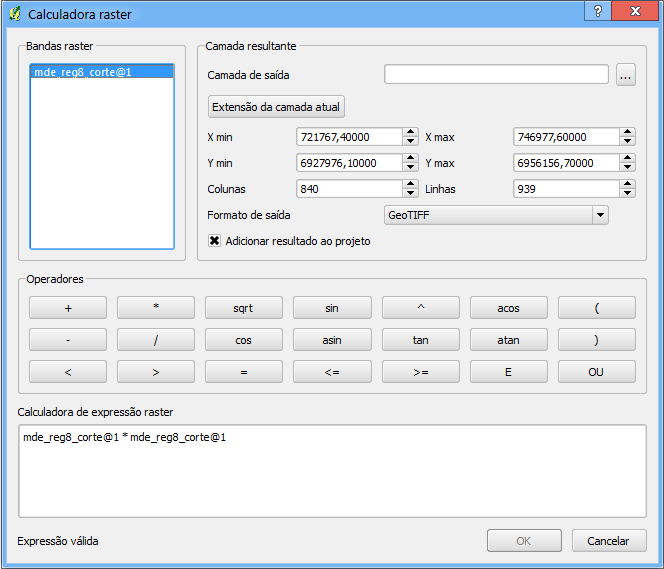
\includegraphics[clip=true, width=11.5cm]{raster_calculator}
%     \caption{Raster Calculator \nixcaption}\label{fig:raster_calculator}
     \caption{Calculatrice raster \nixcaption}\label{fig:raster_calculator}
 \end{figure}

% The \textbf{Fields list} contains all loaded raster layers that can be used. 
% To add a raster to the raster calculator expression field, double
% click its name in the Fields list. You can then use the operators to construct 
% calculation expressions or you can just type it into the box.

La liste \textbf{Bandes Raster} contient toutes les couches rasters actuellement chargées pouvant être utilisé. Pour ajouter un raster à la formule de calcul, faites un double-clic sur son nom dans la liste. Vous pouvez alors utiliser les opérateurs pour construire une formule ou bien les taper directement dans la boîte de saisie.

% In the \textbf{Result layer} section you have to define an output layer. You can 
% then define the extent of the calculation area based on an input raster layer or 
% based on X,Y coordinates and on Columns and Rows to set the resolution of the 
% output layer. If the input layer has a different resolution, the values will be 
% resampled with nearest neighbor algorithm.  
Dans la partie \textbf{Couche de résultat}, vous devez définir la couche en sortie. Vous pouvez préciser l'étendue de la zone de calcul en vous basant sur une couche raster en entrée ou en utilisant des coordonnées X et Y ainsi que des lignes et des colonnes pour indiquer la résolution. Si la couche en entrée a une résolution différence, les valeurs seront interpolées avec l'algorithme du plus proche voisin.

% The \textbf{Operators section} contains all usable operators. To add an operator
% to the raster calculator expression box, click the appropriate button. Mathematical
% calculations ( % , - , * \dots) and trigonometric functions ( sin, cos, tan, \dots) 
% are available. Stay tuned for more operators to come!
La partie \textbf{Opérateurs} contient tous les opérateurs utilisables. Pour ajouter un opérateur à la formule, cliquez sur le bouton approprié. Les calculs mathématiques (+ , - , *,\dots) et les fonctions trigonométriques (sin, cos, tan,\dots) sont disponibles, d'autres feront leur apparition !

% With the \checkbox{Result to project} checkbox the result layer will automatically 
% added to the legend area and can be visualized. 
Le fait de cocher la \checkbox{Ajouter le résultat au projet} chargera automatiquement le raster produit dans votre session pour y être affiché.

%\section{Raster Analysis}\label{sec:raster_analysis}
%\index{Raster!raster analysis}
%\index{Raster analysis}
\section{Analyses raster}\label{sec:raster_analysis}
\index{Raster!raster analysis}
\index{Raster analysis}
%Apart from the raster calculator, additional raster analysis in \qg 1.7 is provided by the GDALTools core plugin. Please refer to section \ref{label_plugingdaltools} for more information.
À part de la calculatrice raster, plus d'analyses rasters dans \qg 1.7 sont fournies par l'extension GDALTools core. Veuillez vous référer à la section \ref{label_plugingdaltools} pour des plus amples informations.

  \FloatBarrier
